\documentclass[twoside]{book}

% Packages required by doxygen
\usepackage{fixltx2e}
\usepackage{calc}
\usepackage{doxygen}
\usepackage[export]{adjustbox} % also loads graphicx
\usepackage{graphicx}
\usepackage[utf8]{inputenc}
\usepackage{makeidx}
\usepackage{multicol}
\usepackage{multirow}
\PassOptionsToPackage{warn}{textcomp}
\usepackage{textcomp}
\usepackage[nointegrals]{wasysym}
\usepackage[table]{xcolor}

% Font selection
\usepackage[T1]{fontenc}
\usepackage[scaled=.90]{helvet}
\usepackage{courier}
\usepackage{amssymb}
\usepackage{sectsty}
\renewcommand{\familydefault}{\sfdefault}
\allsectionsfont{%
  \fontseries{bc}\selectfont%
  \color{darkgray}%
}
\renewcommand{\DoxyLabelFont}{%
  \fontseries{bc}\selectfont%
  \color{darkgray}%
}
\newcommand{\+}{\discretionary{\mbox{\scriptsize$\hookleftarrow$}}{}{}}

% Page & text layout
\usepackage{geometry}
\geometry{%
  a4paper,%
  top=2.5cm,%
  bottom=2.5cm,%
  left=2.5cm,%
  right=2.5cm%
}
\tolerance=750
\hfuzz=15pt
\hbadness=750
\setlength{\emergencystretch}{15pt}
\setlength{\parindent}{0cm}
\setlength{\parskip}{3ex plus 2ex minus 2ex}
\makeatletter
\renewcommand{\paragraph}{%
  \@startsection{paragraph}{4}{0ex}{-1.0ex}{1.0ex}{%
    \normalfont\normalsize\bfseries\SS@parafont%
  }%
}
\renewcommand{\subparagraph}{%
  \@startsection{subparagraph}{5}{0ex}{-1.0ex}{1.0ex}{%
    \normalfont\normalsize\bfseries\SS@subparafont%
  }%
}
\makeatother

% Headers & footers
\usepackage{fancyhdr}
\pagestyle{fancyplain}
\fancyhead[LE]{\fancyplain{}{\bfseries\thepage}}
\fancyhead[CE]{\fancyplain{}{}}
\fancyhead[RE]{\fancyplain{}{\bfseries\leftmark}}
\fancyhead[LO]{\fancyplain{}{\bfseries\rightmark}}
\fancyhead[CO]{\fancyplain{}{}}
\fancyhead[RO]{\fancyplain{}{\bfseries\thepage}}
\fancyfoot[LE]{\fancyplain{}{}}
\fancyfoot[CE]{\fancyplain{}{}}
\fancyfoot[RE]{\fancyplain{}{\bfseries\scriptsize Generated by Doxygen }}
\fancyfoot[LO]{\fancyplain{}{\bfseries\scriptsize Generated by Doxygen }}
\fancyfoot[CO]{\fancyplain{}{}}
\fancyfoot[RO]{\fancyplain{}{}}
\renewcommand{\footrulewidth}{0.4pt}
\renewcommand{\chaptermark}[1]{%
  \markboth{#1}{}%
}
\renewcommand{\sectionmark}[1]{%
  \markright{\thesection\ #1}%
}

% Indices & bibliography
\usepackage{natbib}
\usepackage[titles]{tocloft}
\setcounter{tocdepth}{3}
\setcounter{secnumdepth}{5}
\makeindex

% Hyperlinks (required, but should be loaded last)
\usepackage{ifpdf}
\ifpdf
  \usepackage[pdftex,pagebackref=true]{hyperref}
\else
  \usepackage[ps2pdf,pagebackref=true]{hyperref}
\fi
\hypersetup{%
  colorlinks=true,%
  linkcolor=blue,%
  citecolor=blue,%
  unicode%
}

% Custom commands
\newcommand{\clearemptydoublepage}{%
  \newpage{\pagestyle{empty}\cleardoublepage}%
}

\usepackage{caption}
\captionsetup{labelsep=space,justification=centering,font={bf},singlelinecheck=off,skip=4pt,position=top}

%===== C O N T E N T S =====

\begin{document}

% Titlepage & ToC
\hypersetup{pageanchor=false,
             bookmarksnumbered=true,
             pdfencoding=unicode
            }
\pagenumbering{alph}
\begin{titlepage}
\vspace*{7cm}
\begin{center}%
{\Large My\+Project }\\
\vspace*{1cm}
{\large Generated by Doxygen 1.8.13}\\
\end{center}
\end{titlepage}
\clearemptydoublepage
\pagenumbering{roman}
\tableofcontents
\clearemptydoublepage
\pagenumbering{arabic}
\hypersetup{pageanchor=true}

%--- Begin generated contents ---
\chapter{Hierarchical Index}
\section{Class Hierarchy}
This inheritance list is sorted roughly, but not completely, alphabetically\+:\begin{DoxyCompactList}
\item Action\+Listener\begin{DoxyCompactList}
\item \contentsline{section}{My\+Paint}{\pageref{class_my_paint}}{}
\end{DoxyCompactList}
\item Cloneable\begin{DoxyCompactList}
\item \contentsline{section}{Poly}{\pageref{class_poly}}{}
\end{DoxyCompactList}
\item Float\begin{DoxyCompactList}
\item \contentsline{section}{Z\+Rectangle}{\pageref{class_z_rectangle}}{}
\end{DoxyCompactList}
\item Float\begin{DoxyCompactList}
\item \contentsline{section}{Z\+Ellipse}{\pageref{class_z_ellipse}}{}
\end{DoxyCompactList}
\item J\+Applet\begin{DoxyCompactList}
\item \contentsline{section}{My\+Paint}{\pageref{class_my_paint}}{}
\end{DoxyCompactList}
\item J\+Panel\begin{DoxyCompactList}
\item \contentsline{section}{My\+Panel}{\pageref{class_my_panel}}{}
\end{DoxyCompactList}
\item Mouse\+Listener\begin{DoxyCompactList}
\item \contentsline{section}{My\+Panel}{\pageref{class_my_panel}}{}
\end{DoxyCompactList}
\item Mouse\+Motion\+Listener\begin{DoxyCompactList}
\item \contentsline{section}{My\+Panel}{\pageref{class_my_panel}}{}
\end{DoxyCompactList}
\item Mouse\+Wheel\+Listener\begin{DoxyCompactList}
\item \contentsline{section}{My\+Panel}{\pageref{class_my_panel}}{}
\end{DoxyCompactList}
\item Polygon\begin{DoxyCompactList}
\item \contentsline{section}{Poly}{\pageref{class_poly}}{}
\end{DoxyCompactList}
\item Serializable\begin{DoxyCompactList}
\item \contentsline{section}{Poly}{\pageref{class_poly}}{}
\end{DoxyCompactList}
\item Shape\begin{DoxyCompactList}
\item \contentsline{section}{Poly}{\pageref{class_poly}}{}
\end{DoxyCompactList}
\end{DoxyCompactList}

\chapter{Class Index}
\section{Class List}
Here are the classes, structs, unions and interfaces with brief descriptions\+:\begin{DoxyCompactList}
\item\contentsline{section}{\hyperlink{class_my_paint}{My\+Paint} }{\pageref{class_my_paint}}{}
\item\contentsline{section}{\hyperlink{class_my_panel}{My\+Panel} }{\pageref{class_my_panel}}{}
\item\contentsline{section}{\hyperlink{class_poly}{Poly} }{\pageref{class_poly}}{}
\item\contentsline{section}{\hyperlink{class_z_ellipse}{Z\+Ellipse} }{\pageref{class_z_ellipse}}{}
\item\contentsline{section}{\hyperlink{class_z_rectangle}{Z\+Rectangle} }{\pageref{class_z_rectangle}}{}
\end{DoxyCompactList}

\chapter{Class Documentation}
\hypertarget{class_my_paint}{}\section{My\+Paint Class Reference}
\label{class_my_paint}\index{My\+Paint@{My\+Paint}}
Inheritance diagram for My\+Paint\+:\begin{figure}[H]
\begin{center}
\leavevmode
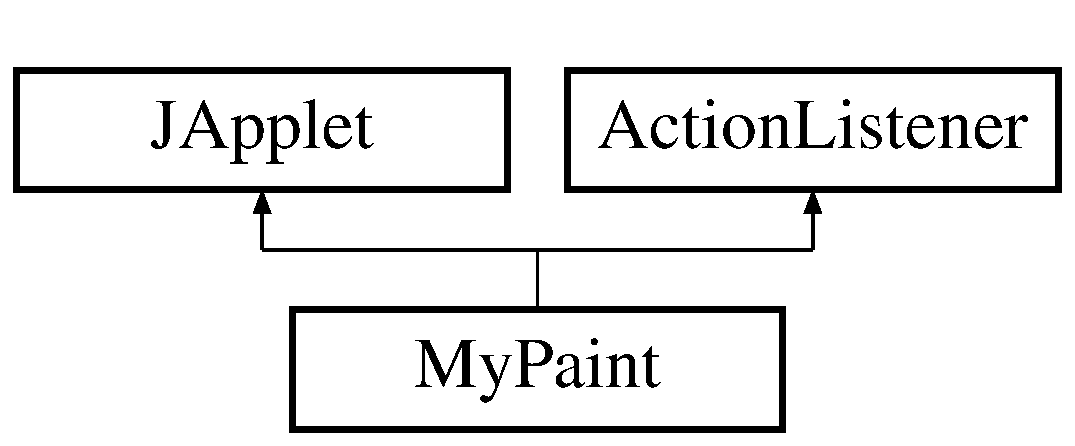
\includegraphics[height=2.000000cm]{class_my_paint}
\end{center}
\end{figure}
\subsection*{Classes}
\begin{DoxyCompactItemize}
\item 
class {\bfseries Dialog}
\item 
class {\bfseries menu\+Applet\+Window\+Adapter}
\item 
class {\bfseries My\+Panel}
\end{DoxyCompactItemize}
\subsection*{Public Member Functions}
\begin{DoxyCompactItemize}
\item 
void \hyperlink{class_my_paint_a215b06cf6775c850921de5180ea65415}{init} ()
\item 
void \hyperlink{class_my_paint_accad3defca48e5a0b34dc2bd3931a183}{action\+Performed} (Action\+Event e)
\end{DoxyCompactItemize}
\subsection*{Private Attributes}
\begin{DoxyCompactItemize}
\item 
Menu\+Bar \hyperlink{class_my_paint_a0484d7171ca748f1b39619fac6b97c29}{my\+Menu}
\item 
Menu \hyperlink{class_my_paint_a9544a7124c7b807531283b3226175b59}{menu1}
\item 
Menu\+Item \hyperlink{class_my_paint_a5f26a81460c19643fbad427c327e87dd}{i0}
\item 
J\+Dialog \hyperlink{class_my_paint_a117ac196604e9160d5d572d97744e528}{my\+Dialog}
\end{DoxyCompactItemize}


\subsection{Detailed Description}
\hyperlink{class_my_paint}{My\+Paint} program to applet do rysowania figur. Pozwala na zmiane ich rozmiaru oraz miejsca i koloru. \begin{DoxyAuthor}{Author}
Volha Hutouskaya 
\end{DoxyAuthor}


\subsection{Member Function Documentation}
\mbox{\Hypertarget{class_my_paint_accad3defca48e5a0b34dc2bd3931a183}\label{class_my_paint_accad3defca48e5a0b34dc2bd3931a183}} 
\index{My\+Paint@{My\+Paint}!action\+Performed@{action\+Performed}}
\index{action\+Performed@{action\+Performed}!My\+Paint@{My\+Paint}}
\subsubsection{\texorpdfstring{action\+Performed()}{actionPerformed()}}
{\footnotesize\ttfamily void My\+Paint.\+action\+Performed (\begin{DoxyParamCaption}\item[{Action\+Event}]{e }\end{DoxyParamCaption})\hspace{0.3cm}{\ttfamily [inline]}}

Metoda do obslugi menu. Po wybraniu jednej z opcji w meniu zapisuje ja do zmiennej action \hyperlink{}{action} \mbox{\Hypertarget{class_my_paint_a215b06cf6775c850921de5180ea65415}\label{class_my_paint_a215b06cf6775c850921de5180ea65415}} 
\index{My\+Paint@{My\+Paint}!init@{init}}
\index{init@{init}!My\+Paint@{My\+Paint}}
\subsubsection{\texorpdfstring{init()}{init()}}
{\footnotesize\ttfamily void My\+Paint.\+init (\begin{DoxyParamCaption}{ }\end{DoxyParamCaption})\hspace{0.3cm}{\ttfamily [inline]}}

Tworzy \hyperlink{class_my_paint}{My\+Paint} 

\subsection{Member Data Documentation}
\mbox{\Hypertarget{class_my_paint_a5f26a81460c19643fbad427c327e87dd}\label{class_my_paint_a5f26a81460c19643fbad427c327e87dd}} 
\index{My\+Paint@{My\+Paint}!i0@{i0}}
\index{i0@{i0}!My\+Paint@{My\+Paint}}
\subsubsection{\texorpdfstring{i0}{i0}}
{\footnotesize\ttfamily Menu\+Item My\+Paint.\+i0\hspace{0.3cm}{\ttfamily [private]}}

Opcje do wybrania w meniu \mbox{\Hypertarget{class_my_paint_a9544a7124c7b807531283b3226175b59}\label{class_my_paint_a9544a7124c7b807531283b3226175b59}} 
\index{My\+Paint@{My\+Paint}!menu1@{menu1}}
\index{menu1@{menu1}!My\+Paint@{My\+Paint}}
\subsubsection{\texorpdfstring{menu1}{menu1}}
{\footnotesize\ttfamily Menu My\+Paint.\+menu1\hspace{0.3cm}{\ttfamily [private]}}

Menu i Podmenu appleta \mbox{\Hypertarget{class_my_paint_a117ac196604e9160d5d572d97744e528}\label{class_my_paint_a117ac196604e9160d5d572d97744e528}} 
\index{My\+Paint@{My\+Paint}!my\+Dialog@{my\+Dialog}}
\index{my\+Dialog@{my\+Dialog}!My\+Paint@{My\+Paint}}
\subsubsection{\texorpdfstring{my\+Dialog}{myDialog}}
{\footnotesize\ttfamily J\+Dialog My\+Paint.\+my\+Dialog\hspace{0.3cm}{\ttfamily [private]}}

Okno dialogowe, zawiera informacje o programie \mbox{\Hypertarget{class_my_paint_a0484d7171ca748f1b39619fac6b97c29}\label{class_my_paint_a0484d7171ca748f1b39619fac6b97c29}} 
\index{My\+Paint@{My\+Paint}!my\+Menu@{my\+Menu}}
\index{my\+Menu@{my\+Menu}!My\+Paint@{My\+Paint}}
\subsubsection{\texorpdfstring{my\+Menu}{myMenu}}
{\footnotesize\ttfamily Menu\+Bar My\+Paint.\+my\+Menu\hspace{0.3cm}{\ttfamily [private]}}

Menu\+Bar appleta 

The documentation for this class was generated from the following file\+:\begin{DoxyCompactItemize}
\item 
D\+:/job/semestr2/lab/\+A/My\+Paint.\+java\end{DoxyCompactItemize}

\hypertarget{class_my_panel}{}\section{My\+Panel Class Reference}
\label{class_my_panel}\index{My\+Panel@{My\+Panel}}
Inheritance diagram for My\+Panel\+:\begin{figure}[H]
\begin{center}
\leavevmode
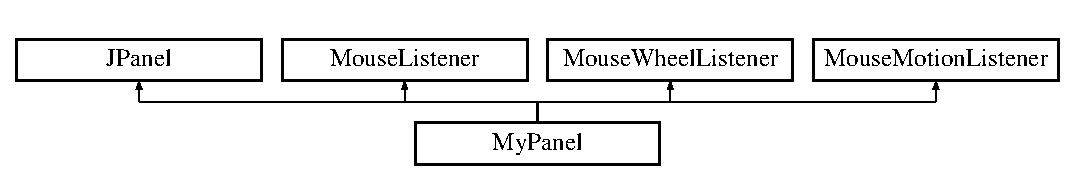
\includegraphics[height=1.985816cm]{class_my_panel}
\end{center}
\end{figure}
\subsection*{Public Member Functions}
\begin{DoxyCompactItemize}
\item 
\hyperlink{class_my_panel_a9395d78dbd3ccb9159bcdfd8fa54bf62}{My\+Panel} ()
\item 
void \hyperlink{class_my_panel_a01d8184b14a097e845b1845ddf3e4d7d}{paint\+Component} (Graphics g)
\item 
void \hyperlink{class_my_panel_a081232045c04ce6f009f19b500062c91}{change\+Color} (Color co)
\item 
\mbox{\Hypertarget{class_my_panel_ad1ac4015693658076ffa37d8d3cc16dc}\label{class_my_panel_ad1ac4015693658076ffa37d8d3cc16dc}} 
void {\bfseries mouse\+Pressed} (Mouse\+Event e)
\item 
void \hyperlink{class_my_panel_a5d9496e3a6fcc77da4edb2ead258f286}{poly\+Function} (Array\+List$<$ Point2\+D.\+Float $>$ points)
\item 
\mbox{\Hypertarget{class_my_panel_a89449fea451e2350cdec8bd638d36344}\label{class_my_panel_a89449fea451e2350cdec8bd638d36344}} 
void {\bfseries mouse\+Dragged} (Mouse\+Event e)
\item 
\mbox{\Hypertarget{class_my_panel_ad512efaf729c549e397b58498bff6043}\label{class_my_panel_ad512efaf729c549e397b58498bff6043}} 
void {\bfseries mouse\+Wheel\+Moved} (Mouse\+Wheel\+Event e)
\item 
\mbox{\Hypertarget{class_my_panel_ae26f94cb4b562a2c26928914de71b76e}\label{class_my_panel_ae26f94cb4b562a2c26928914de71b76e}} 
void {\bfseries mouse\+Moved} (Mouse\+Event e)
\item 
\mbox{\Hypertarget{class_my_panel_afaf9c657c61bebb715330371b17b9852}\label{class_my_panel_afaf9c657c61bebb715330371b17b9852}} 
void {\bfseries mouse\+Entered} (Mouse\+Event e)
\item 
\mbox{\Hypertarget{class_my_panel_a86b4f660c427fa44902e777f26d5ea54}\label{class_my_panel_a86b4f660c427fa44902e777f26d5ea54}} 
void {\bfseries mouse\+Exited} (Mouse\+Event e)
\item 
\mbox{\Hypertarget{class_my_panel_a657ce352f2f06f2cf535b08019849bef}\label{class_my_panel_a657ce352f2f06f2cf535b08019849bef}} 
void {\bfseries mouse\+Clicked} (Mouse\+Event e)
\item 
\mbox{\Hypertarget{class_my_panel_a975c43d6d03a6dce44f1791bce757839}\label{class_my_panel_a975c43d6d03a6dce44f1791bce757839}} 
void {\bfseries mouse\+Released} (Mouse\+Event e)
\end{DoxyCompactItemize}
\subsection*{Public Attributes}
\begin{DoxyCompactItemize}
\item 
J\+Popup\+Menu \hyperlink{class_my_panel_a5214776606bc8c37c7a8395827a0067b}{menu}
\end{DoxyCompactItemize}
\subsection*{Private Member Functions}
\begin{DoxyCompactItemize}
\item 
\mbox{\Hypertarget{class_my_panel_af5f17fcefe8341ad03e7d60d38601af1}\label{class_my_panel_af5f17fcefe8341ad03e7d60d38601af1}} 
void {\bfseries check\+Menu} (Mouse\+Event e)
\item 
void \hyperlink{class_my_panel_add2eb62a2206dc06b714021d160443eb}{change\+Active\+Figures} (int x, int y)
\item 
void \hyperlink{class_my_panel_a87b36d0049d583ddb1d8369a2d026af2}{get\+Rid\+Of\+Active\+Figures} ()
\item 
void \hyperlink{class_my_panel_aa5aa1bff3cdad750439efd1a6c0b7a94}{add\+To\+List} (float x\+Pressed, float y\+Pressed, float width, float hight)
\item 
void \hyperlink{class_my_panel_a9a082d14cf56b66e9899928d01b2018f}{do\+Move} (Mouse\+Event e)
\item 
void \hyperlink{class_my_panel_a557eeac694b8daa3a7da493d62434533}{do\+Scale} (Mouse\+Wheel\+Event e)
\end{DoxyCompactItemize}


\subsection{Detailed Description}
Klasa w ktorej odbywa sie rysowanie

\begin{DoxyAuthor}{Author}
Volha Hutouskaya 
\end{DoxyAuthor}


\subsection{Constructor \& Destructor Documentation}
\mbox{\Hypertarget{class_my_panel_a9395d78dbd3ccb9159bcdfd8fa54bf62}\label{class_my_panel_a9395d78dbd3ccb9159bcdfd8fa54bf62}} 
\index{My\+Panel@{My\+Panel}!My\+Panel@{My\+Panel}}
\index{My\+Panel@{My\+Panel}!My\+Panel@{My\+Panel}}
\subsubsection{\texorpdfstring{My\+Panel()}{MyPanel()}}
{\footnotesize\ttfamily My\+Panel.\+My\+Panel (\begin{DoxyParamCaption}{ }\end{DoxyParamCaption})\hspace{0.3cm}{\ttfamily [inline]}}

Tworzy nowy objekt. 

\subsection{Member Function Documentation}
\mbox{\Hypertarget{class_my_panel_aa5aa1bff3cdad750439efd1a6c0b7a94}\label{class_my_panel_aa5aa1bff3cdad750439efd1a6c0b7a94}} 
\index{My\+Panel@{My\+Panel}!add\+To\+List@{add\+To\+List}}
\index{add\+To\+List@{add\+To\+List}!My\+Panel@{My\+Panel}}
\subsubsection{\texorpdfstring{add\+To\+List()}{addToList()}}
{\footnotesize\ttfamily void My\+Panel.\+add\+To\+List (\begin{DoxyParamCaption}\item[{float}]{x\+Pressed,  }\item[{float}]{y\+Pressed,  }\item[{float}]{width,  }\item[{float}]{hight }\end{DoxyParamCaption})\hspace{0.3cm}{\ttfamily [inline]}, {\ttfamily [private]}}

Metoda dodajaca okragi i prostokaty do list. 
\begin{DoxyParams}{Parameters}
{\em x\+Pressed} & wspolrzedna x klikniecia \\
\hline
{\em y\+Pressed} & wspolrzedna y klikniecia \\
\hline
{\em width} & szerokosc figury \hyperlink{}{width} \\
\hline
{\em hight} & wysokosc figury \hyperlink{}{hight} \\
\hline
\end{DoxyParams}
\mbox{\Hypertarget{class_my_panel_add2eb62a2206dc06b714021d160443eb}\label{class_my_panel_add2eb62a2206dc06b714021d160443eb}} 
\index{My\+Panel@{My\+Panel}!change\+Active\+Figures@{change\+Active\+Figures}}
\index{change\+Active\+Figures@{change\+Active\+Figures}!My\+Panel@{My\+Panel}}
\subsubsection{\texorpdfstring{change\+Active\+Figures()}{changeActiveFigures()}}
{\footnotesize\ttfamily void My\+Panel.\+change\+Active\+Figures (\begin{DoxyParamCaption}\item[{int}]{x,  }\item[{int}]{y }\end{DoxyParamCaption})\hspace{0.3cm}{\ttfamily [inline]}, {\ttfamily [private]}}

Metoda zmieniajca aktywnosc figury \mbox{\Hypertarget{class_my_panel_a081232045c04ce6f009f19b500062c91}\label{class_my_panel_a081232045c04ce6f009f19b500062c91}} 
\index{My\+Panel@{My\+Panel}!change\+Color@{change\+Color}}
\index{change\+Color@{change\+Color}!My\+Panel@{My\+Panel}}
\subsubsection{\texorpdfstring{change\+Color()}{changeColor()}}
{\footnotesize\ttfamily void My\+Panel.\+change\+Color (\begin{DoxyParamCaption}\item[{Color}]{co }\end{DoxyParamCaption})\hspace{0.3cm}{\ttfamily [inline]}}

Metoda zmieniajca kolor aktywnej figury 
\begin{DoxyParams}{Parameters}
{\em co} & kolor \\
\hline
\end{DoxyParams}
\mbox{\Hypertarget{class_my_panel_a9a082d14cf56b66e9899928d01b2018f}\label{class_my_panel_a9a082d14cf56b66e9899928d01b2018f}} 
\index{My\+Panel@{My\+Panel}!do\+Move@{do\+Move}}
\index{do\+Move@{do\+Move}!My\+Panel@{My\+Panel}}
\subsubsection{\texorpdfstring{do\+Move()}{doMove()}}
{\footnotesize\ttfamily void My\+Panel.\+do\+Move (\begin{DoxyParamCaption}\item[{Mouse\+Event}]{e }\end{DoxyParamCaption})\hspace{0.3cm}{\ttfamily [inline]}, {\ttfamily [private]}}

Metoda do przemieszczania figur \mbox{\Hypertarget{class_my_panel_a557eeac694b8daa3a7da493d62434533}\label{class_my_panel_a557eeac694b8daa3a7da493d62434533}} 
\index{My\+Panel@{My\+Panel}!do\+Scale@{do\+Scale}}
\index{do\+Scale@{do\+Scale}!My\+Panel@{My\+Panel}}
\subsubsection{\texorpdfstring{do\+Scale()}{doScale()}}
{\footnotesize\ttfamily void My\+Panel.\+do\+Scale (\begin{DoxyParamCaption}\item[{Mouse\+Wheel\+Event}]{e }\end{DoxyParamCaption})\hspace{0.3cm}{\ttfamily [inline]}, {\ttfamily [private]}}

Metoda do skalowania figur \mbox{\Hypertarget{class_my_panel_a87b36d0049d583ddb1d8369a2d026af2}\label{class_my_panel_a87b36d0049d583ddb1d8369a2d026af2}} 
\index{My\+Panel@{My\+Panel}!get\+Rid\+Of\+Active\+Figures@{get\+Rid\+Of\+Active\+Figures}}
\index{get\+Rid\+Of\+Active\+Figures@{get\+Rid\+Of\+Active\+Figures}!My\+Panel@{My\+Panel}}
\subsubsection{\texorpdfstring{get\+Rid\+Of\+Active\+Figures()}{getRidOfActiveFigures()}}
{\footnotesize\ttfamily void My\+Panel.\+get\+Rid\+Of\+Active\+Figures (\begin{DoxyParamCaption}{ }\end{DoxyParamCaption})\hspace{0.3cm}{\ttfamily [inline]}, {\ttfamily [private]}}

Metoda zmieniajca aktywnosc figury przy wybraniu innej opcji w menu. \mbox{\Hypertarget{class_my_panel_a01d8184b14a097e845b1845ddf3e4d7d}\label{class_my_panel_a01d8184b14a097e845b1845ddf3e4d7d}} 
\index{My\+Panel@{My\+Panel}!paint\+Component@{paint\+Component}}
\index{paint\+Component@{paint\+Component}!My\+Panel@{My\+Panel}}
\subsubsection{\texorpdfstring{paint\+Component()}{paintComponent()}}
{\footnotesize\ttfamily void My\+Panel.\+paint\+Component (\begin{DoxyParamCaption}\item[{Graphics}]{g }\end{DoxyParamCaption})\hspace{0.3cm}{\ttfamily [inline]}}

Metoda rysujaca figury i punkty \mbox{\Hypertarget{class_my_panel_a5d9496e3a6fcc77da4edb2ead258f286}\label{class_my_panel_a5d9496e3a6fcc77da4edb2ead258f286}} 
\index{My\+Panel@{My\+Panel}!poly\+Function@{poly\+Function}}
\index{poly\+Function@{poly\+Function}!My\+Panel@{My\+Panel}}
\subsubsection{\texorpdfstring{poly\+Function()}{polyFunction()}}
{\footnotesize\ttfamily void My\+Panel.\+poly\+Function (\begin{DoxyParamCaption}\item[{Array\+List$<$ Point2\+D.\+Float $>$}]{points }\end{DoxyParamCaption})\hspace{0.3cm}{\ttfamily [inline]}}

Metoda tworzaca i dodajaca do listy wielokaty 
\begin{DoxyParams}{Parameters}
{\em points} & lista nacisnietych punktow jednego wielokata w trybie wielokata \\
\hline
\end{DoxyParams}


\subsection{Member Data Documentation}
\mbox{\Hypertarget{class_my_panel_a5214776606bc8c37c7a8395827a0067b}\label{class_my_panel_a5214776606bc8c37c7a8395827a0067b}} 
\index{My\+Panel@{My\+Panel}!menu@{menu}}
\index{menu@{menu}!My\+Panel@{My\+Panel}}
\subsubsection{\texorpdfstring{menu}{menu}}
{\footnotesize\ttfamily J\+Popup\+Menu My\+Panel.\+menu}

Wyskakujące menu. Sluzy do zmiany kolorow. 

The documentation for this class was generated from the following file\+:\begin{DoxyCompactItemize}
\item 
D\+:/job/semestr2/lab/\+A/My\+Panel.\+java\end{DoxyCompactItemize}

\hypertarget{class_poly}{}\section{Poly Class Reference}
\label{class_poly}\index{Poly@{Poly}}
Inheritance diagram for Poly\+:\begin{figure}[H]
\begin{center}
\leavevmode
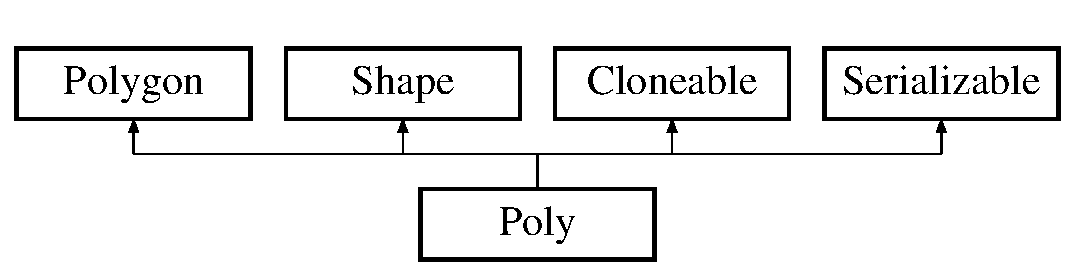
\includegraphics[height=2.000000cm]{class_poly}
\end{center}
\end{figure}
\subsection*{Public Member Functions}
\begin{DoxyCompactItemize}
\item 
\mbox{\Hypertarget{class_poly_ad24cfd4743b10e900bca1c2c2cabf3af}\label{class_poly_ad24cfd4743b10e900bca1c2c2cabf3af}} 
{\bfseries Poly} (int\mbox{[}$\,$\mbox{]} x, int\mbox{[}$\,$\mbox{]} y, int n)
\item 
\mbox{\Hypertarget{class_poly_abe407318f79cd8fbed337334bdfdc6f9}\label{class_poly_abe407318f79cd8fbed337334bdfdc6f9}} 
void {\bfseries change\+Active} ()
\item 
\mbox{\Hypertarget{class_poly_a8a1eca3567a02fa17eec76e3282eb1e1}\label{class_poly_a8a1eca3567a02fa17eec76e3282eb1e1}} 
boolean {\bfseries is\+Active} ()
\item 
\mbox{\Hypertarget{class_poly_afb1e52dd476370cff30d63e2ac9768fa}\label{class_poly_afb1e52dd476370cff30d63e2ac9768fa}} 
Color {\bfseries get\+Color} ()
\item 
\mbox{\Hypertarget{class_poly_a71acefcfe7fb0ea8100f2cf2617578ff}\label{class_poly_a71acefcfe7fb0ea8100f2cf2617578ff}} 
void {\bfseries change\+Color} (Color c)
\item 
\mbox{\Hypertarget{class_poly_a3e2d7553c1061c4c51ab2b49824e4ca8}\label{class_poly_a3e2d7553c1061c4c51ab2b49824e4ca8}} 
boolean {\bfseries is\+Hit} (int x, int y)
\item 
\mbox{\Hypertarget{class_poly_af0e6bae618f0ce57e6e9e3cd3cc0c06f}\label{class_poly_af0e6bae618f0ce57e6e9e3cd3cc0c06f}} 
void {\bfseries addX} (int x)
\item 
\mbox{\Hypertarget{class_poly_a411d0d5e8618d1b31a2c9d412299ff60}\label{class_poly_a411d0d5e8618d1b31a2c9d412299ff60}} 
void {\bfseries addY} (int y)
\item 
\mbox{\Hypertarget{class_poly_a0b7b6b3fff39f8db9d136262d69a9248}\label{class_poly_a0b7b6b3fff39f8db9d136262d69a9248}} 
void {\bfseries scaling} (float w)
\item 
\mbox{\Hypertarget{class_poly_aab4ca8dc1db70a4d3696227ee17ef42f}\label{class_poly_aab4ca8dc1db70a4d3696227ee17ef42f}} 
int {\bfseries find\+CenterX} ()
\item 
\mbox{\Hypertarget{class_poly_a267142033abf00fb96a8b2d3aefc920d}\label{class_poly_a267142033abf00fb96a8b2d3aefc920d}} 
int {\bfseries find\+CenterY} ()
\end{DoxyCompactItemize}
\subsection*{Private Attributes}
\begin{DoxyCompactItemize}
\item 
\mbox{\Hypertarget{class_poly_af7a3aa122a5eaf1bf3d9eb95750ce536}\label{class_poly_af7a3aa122a5eaf1bf3d9eb95750ce536}} 
boolean {\bfseries active} = false
\item 
\mbox{\Hypertarget{class_poly_a8fa0ee493b8d5c0d20612acee885b3a9}\label{class_poly_a8fa0ee493b8d5c0d20612acee885b3a9}} 
Color {\bfseries color} = Color.\+B\+L\+A\+CK
\end{DoxyCompactItemize}


\subsection{Detailed Description}
Klasa przechowywujaca dane wielokata.

\begin{DoxyAuthor}{Author}
Volha Hutouskaya 
\end{DoxyAuthor}


The documentation for this class was generated from the following file\+:\begin{DoxyCompactItemize}
\item 
D\+:/job/semestr2/lab/\+A/Poly.\+java\end{DoxyCompactItemize}

\hypertarget{class_z_ellipse}{}\section{Z\+Ellipse Class Reference}
\label{class_z_ellipse}\index{Z\+Ellipse@{Z\+Ellipse}}
Inheritance diagram for Z\+Ellipse\+:\begin{figure}[H]
\begin{center}
\leavevmode
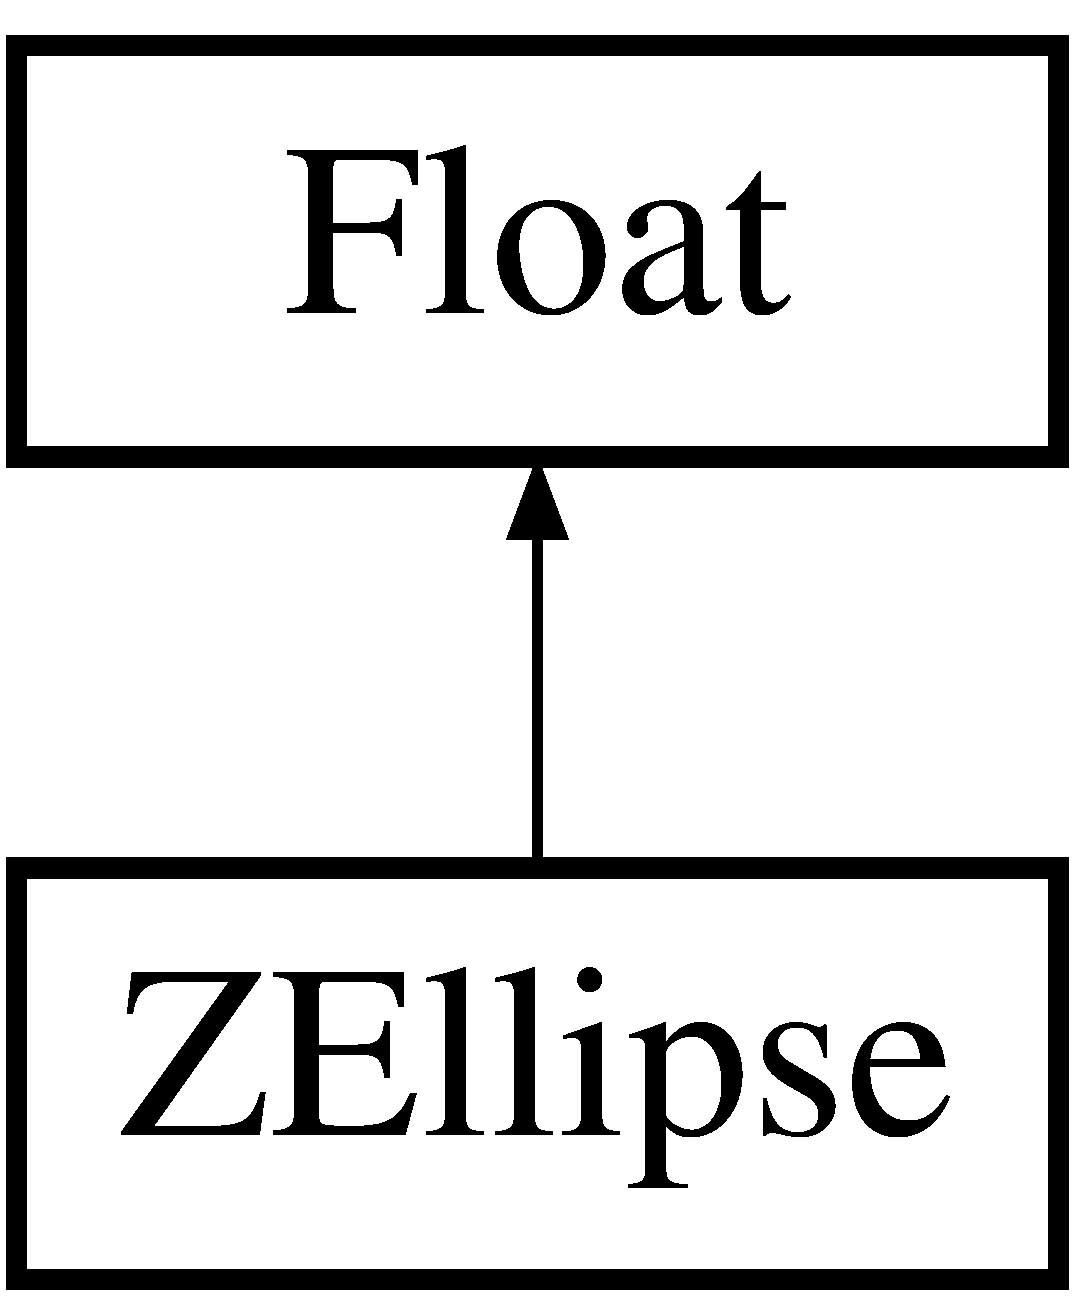
\includegraphics[height=2.000000cm]{class_z_ellipse}
\end{center}
\end{figure}
\subsection*{Public Member Functions}
\begin{DoxyCompactItemize}
\item 
\mbox{\Hypertarget{class_z_ellipse_ae0c643fe69b8daaa92fedb71d343c2c2}\label{class_z_ellipse_ae0c643fe69b8daaa92fedb71d343c2c2}} 
{\bfseries Z\+Ellipse} (float x, float y, float width, float height)
\item 
\mbox{\Hypertarget{class_z_ellipse_a1e4d268bc44ca7d86bfe6ee56614270e}\label{class_z_ellipse_a1e4d268bc44ca7d86bfe6ee56614270e}} 
void {\bfseries change\+Active} ()
\item 
\mbox{\Hypertarget{class_z_ellipse_a12fccf373e68bedfe75ca4de6b442157}\label{class_z_ellipse_a12fccf373e68bedfe75ca4de6b442157}} 
boolean {\bfseries is\+Active} ()
\item 
\mbox{\Hypertarget{class_z_ellipse_a71b85d8bf2da93f76cb8fd250d14086e}\label{class_z_ellipse_a71b85d8bf2da93f76cb8fd250d14086e}} 
Color {\bfseries get\+Color} ()
\item 
\mbox{\Hypertarget{class_z_ellipse_a81e08ad0fd085a1f06ef39b26403b9b7}\label{class_z_ellipse_a81e08ad0fd085a1f06ef39b26403b9b7}} 
void {\bfseries change\+Color} (Color c)
\item 
\mbox{\Hypertarget{class_z_ellipse_acade6d1a85051ec181e916b77ec47d19}\label{class_z_ellipse_acade6d1a85051ec181e916b77ec47d19}} 
boolean {\bfseries is\+Hit} (int x, int y)
\item 
\mbox{\Hypertarget{class_z_ellipse_ae3273269cea9b18ed643d858ff92906f}\label{class_z_ellipse_ae3273269cea9b18ed643d858ff92906f}} 
void {\bfseries addX} (float x)
\item 
\mbox{\Hypertarget{class_z_ellipse_aa2c979d23313a02418be0d6b7a98778f}\label{class_z_ellipse_aa2c979d23313a02418be0d6b7a98778f}} 
void {\bfseries addY} (float y)
\item 
\mbox{\Hypertarget{class_z_ellipse_a0556391e87d9bad231ea415aec9beed8}\label{class_z_ellipse_a0556391e87d9bad231ea415aec9beed8}} 
void {\bfseries add\+Width} (float w)
\item 
\mbox{\Hypertarget{class_z_ellipse_a32d292e4f1d950cd3277a22a35ae8ab6}\label{class_z_ellipse_a32d292e4f1d950cd3277a22a35ae8ab6}} 
void {\bfseries add\+Height} (float h)
\end{DoxyCompactItemize}
\subsection*{Private Attributes}
\begin{DoxyCompactItemize}
\item 
\mbox{\Hypertarget{class_z_ellipse_a5f83cf624b9d618d39a314bf529cbbfc}\label{class_z_ellipse_a5f83cf624b9d618d39a314bf529cbbfc}} 
boolean {\bfseries active} = false
\item 
\mbox{\Hypertarget{class_z_ellipse_a030e36cd26072ad233c827d2772ab275}\label{class_z_ellipse_a030e36cd26072ad233c827d2772ab275}} 
Color {\bfseries color} = Color.\+B\+L\+A\+CK
\end{DoxyCompactItemize}


\subsection{Detailed Description}
Klasa przechowywujaca dane okrogow.

\begin{DoxyAuthor}{Author}
Volha Hutouskaya 
\end{DoxyAuthor}


The documentation for this class was generated from the following file\+:\begin{DoxyCompactItemize}
\item 
D\+:/job/semestr2/lab/\+A/Z\+Ellipse.\+java\end{DoxyCompactItemize}

\hypertarget{class_z_rectangle}{}\section{Z\+Rectangle Class Reference}
\label{class_z_rectangle}\index{Z\+Rectangle@{Z\+Rectangle}}
Inheritance diagram for Z\+Rectangle\+:\begin{figure}[H]
\begin{center}
\leavevmode
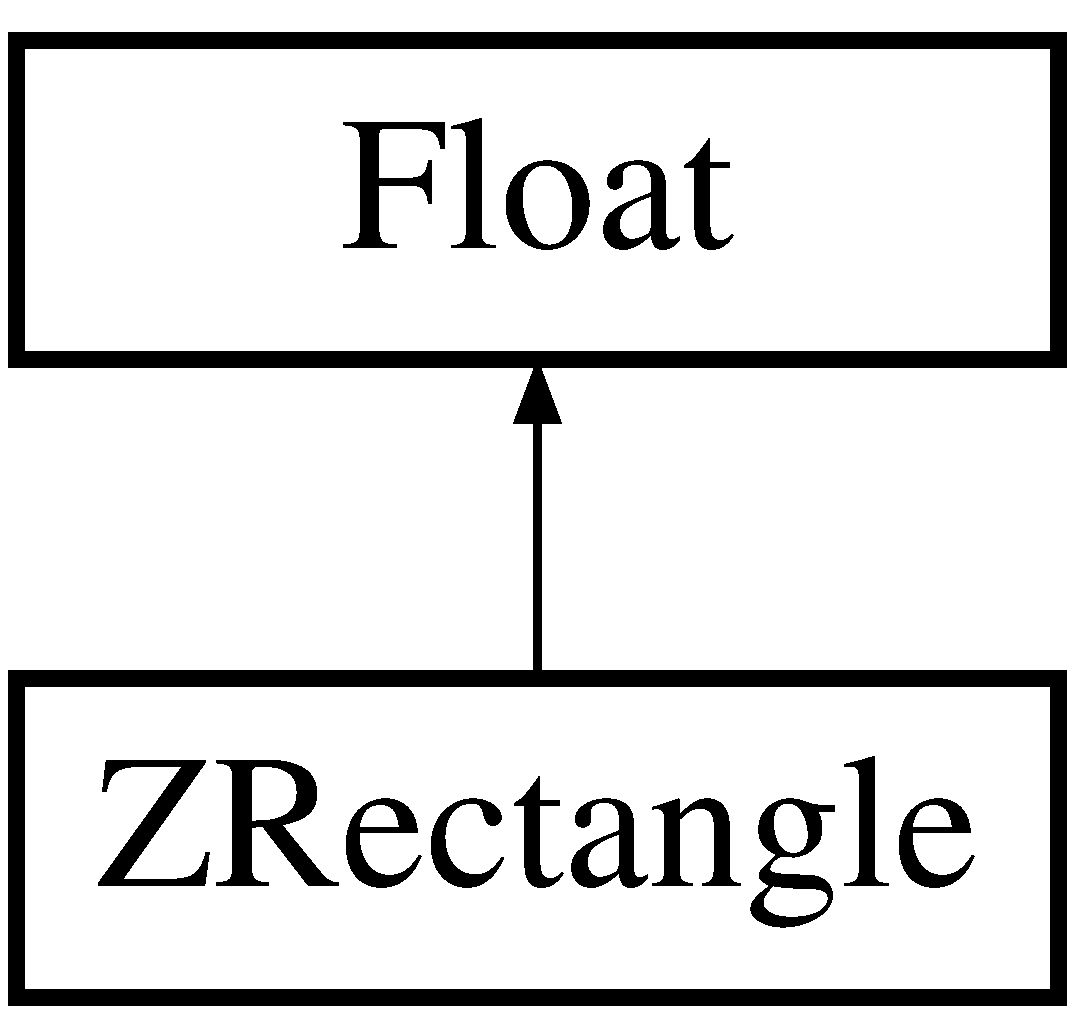
\includegraphics[height=2.000000cm]{class_z_rectangle}
\end{center}
\end{figure}
\subsection*{Public Member Functions}
\begin{DoxyCompactItemize}
\item 
\mbox{\Hypertarget{class_z_rectangle_acee0e23b738a3ad9ac81b03bb1926f20}\label{class_z_rectangle_acee0e23b738a3ad9ac81b03bb1926f20}} 
{\bfseries Z\+Rectangle} (float x, float y, float width, float height)
\item 
\mbox{\Hypertarget{class_z_rectangle_a8c0726c0ad8dac001dfb140725e053dc}\label{class_z_rectangle_a8c0726c0ad8dac001dfb140725e053dc}} 
void {\bfseries change\+Active} ()
\item 
\mbox{\Hypertarget{class_z_rectangle_a282cd5d7d28589d69eec4b1b300a68ee}\label{class_z_rectangle_a282cd5d7d28589d69eec4b1b300a68ee}} 
boolean {\bfseries is\+Active} ()
\item 
\mbox{\Hypertarget{class_z_rectangle_ae93e72310763ef5c8cf986ee8742871c}\label{class_z_rectangle_ae93e72310763ef5c8cf986ee8742871c}} 
Color {\bfseries get\+Color} ()
\item 
\mbox{\Hypertarget{class_z_rectangle_ad35584292b4e8f0381a57f71d8a1ac22}\label{class_z_rectangle_ad35584292b4e8f0381a57f71d8a1ac22}} 
void {\bfseries change\+Color} (Color c)
\item 
\mbox{\Hypertarget{class_z_rectangle_a4fafc725bd2d528a4c461308a6551831}\label{class_z_rectangle_a4fafc725bd2d528a4c461308a6551831}} 
boolean {\bfseries is\+Hit} (int x, int y)
\item 
\mbox{\Hypertarget{class_z_rectangle_a0a86d4da2bb5cf38a67f2383281e87d9}\label{class_z_rectangle_a0a86d4da2bb5cf38a67f2383281e87d9}} 
void {\bfseries addX} (float x)
\item 
\mbox{\Hypertarget{class_z_rectangle_aa1479d07a461ed586c2a5413e8f4677b}\label{class_z_rectangle_aa1479d07a461ed586c2a5413e8f4677b}} 
void {\bfseries addY} (float y)
\item 
\mbox{\Hypertarget{class_z_rectangle_abb3d81ce739819f51168418e2ac14c06}\label{class_z_rectangle_abb3d81ce739819f51168418e2ac14c06}} 
void {\bfseries add\+Width} (float w)
\item 
\mbox{\Hypertarget{class_z_rectangle_ae849086a6b72b6ecd087c9ebc783bd01}\label{class_z_rectangle_ae849086a6b72b6ecd087c9ebc783bd01}} 
void {\bfseries add\+Height} (float h)
\end{DoxyCompactItemize}
\subsection*{Private Attributes}
\begin{DoxyCompactItemize}
\item 
\mbox{\Hypertarget{class_z_rectangle_a26796b0689b4c9697b279d80e6bd3165}\label{class_z_rectangle_a26796b0689b4c9697b279d80e6bd3165}} 
boolean {\bfseries active} = false
\item 
\mbox{\Hypertarget{class_z_rectangle_abdd8c9c5e161fd801f22f4c3333192e3}\label{class_z_rectangle_abdd8c9c5e161fd801f22f4c3333192e3}} 
Color {\bfseries color} = Color.\+B\+L\+A\+CK
\end{DoxyCompactItemize}


\subsection{Detailed Description}
Klasa przechowywujaca dane prostokatow.

\begin{DoxyAuthor}{Author}
Volha Hutouskaya 
\end{DoxyAuthor}


The documentation for this class was generated from the following file\+:\begin{DoxyCompactItemize}
\item 
D\+:/job/semestr2/lab/\+A/Z\+Rectangle.\+java\end{DoxyCompactItemize}

%--- End generated contents ---

% Index
\backmatter
\newpage
\phantomsection
\clearemptydoublepage
\addcontentsline{toc}{chapter}{Index}
\printindex

\end{document}
